\documentclass[draft]{article}
\usepackage{subcaption}
\usepackage{float}
\usepackage{graphicx}
\usepackage[backend=biber]{biblatex}
\addbibresource{citations.bib}
% \usepackage{pdfpages}
\usepackage[left=1.25in, top=1in, bottom=1in, right=0.9in]{geometry}
\usepackage{enumitem}
\usepackage{setspace}
\usepackage{parskip}
\setlength{\parskip}{1em}
\usepackage{hyperref}

\doublespacing

\title{Case Study: Disk Management}
\author{Darshan Shrestha}
\date{July 2026}

\begin{document}

\maketitle

\newpage
\section*{Abstract}

Context — One sentence on the broader topic. Why does storage technology matter?

Purpose — What is this case study trying to do? (Similar to your objective, but shorter.)

Scope — What technologies or areas does it cover? (HDD, SSD, NVMe)

Key Findings — What did you discover or conclude from your study?

Conclusion / Significance — Why does it matter? What's the takeaway?

\textbf{Keywords:} Hard Disk Drive (HDD), Magnetic Storage, Disk Management, Operating Systems, Disk Scheduling, Secondary Memory.

\newpage
\tableofcontents


\newpage
\section{Introduction}
Storage is one of the most important components of any computing system. From the earliest days of computing to the modern cloud era, the ability to store and retrieve data efficiently has been critical to how computers function. As applications have grown more complex and data volumes have exploded, the demand for faster, more reliable, and more cost-effective storage solutions has never been greater.


Over the decades, three major disk storage technologies have emerged and evolved: the Hard Disk Drive (HDD), the Solid State Drive (SSD), and the NVMe (Non-Volatile Memory Express) drive. Each represents a leap forward in storage performance, and each comes with its own set of trade-offs in terms of speed, cost, capacity, and durability.


From an operating system perspective, storage management is a core responsibility. The OS must communicate with storage devices through device drivers, manage how data is read and written through I/O scheduling algorithms, and organize data through file systems. The type of storage device used significantly affects how these processes are carried out and how efficiently the overall system performs.


This case study examines the architecture, working principles, and performance characteristics of HDD, SSD, and NVMe technologies. It further explores how the operating system interacts with each of these storage types, and analyzes the real-world scenarios in which each technology is most appropriately used. By the end of this study, the reader will have a clear understanding of how disk storage technologies have evolved and why choosing the right storage medium matters in modern computing.

\section{Objective}

The objective of this case study is to understand how different disk storage technologies — HDD, SSD, and NVMe — are managed by the operating system, exploring how device drivers, I/O scheduling, and file systems are designed to interact with each storage medium to optimize system performance

\newpage
\section{Hard Disk Drive (HDD) Technology}

A Hard Disk Drive (HDD) is an electro-mechanical, non-volatile computer data storage device that utilizes magnetic storage to store and retrieve digital data \cite{wiki_hdd}. Unlike volatile RAM, HDDs retain data even when the power is turned off, making them the primary choice for long-term storage of operating systems, applications, and user files \cite{gfg_hdd_memory, gfg_storage_structure}.

\subsection{Physical Infrastructure}


\begin{enumerate}[label=\roman*.]
    \item \textbf{Platters and Spindle:} The physical structure of an HDD consists of rigid, rapidly rotating circular disks called platters, which are coated with magnetic material \cite{wiki_hdd, gfg_hdd_memory}.

    \item \textbf{Read/Write Heads:} Data is accessed via read/write heads positioned on a moving actuator arm that traverses the platter surfaces in a random-access manner, allowing individual blocks of data to be retrieved in any order \cite{wiki_hdd, gfg_hdd_memory}.
    
    \item \textbf{Mechanical Speed:} These platters are mounted on a central spindle that rotates at high speeds, typically ranging from 4,200 to 15,000 RPM \cite{gfg_hdd_memory, wiki_hdd}.
    
\end{enumerate}


\vspace{1 in}
\begin{figure}[H]
    \centering
    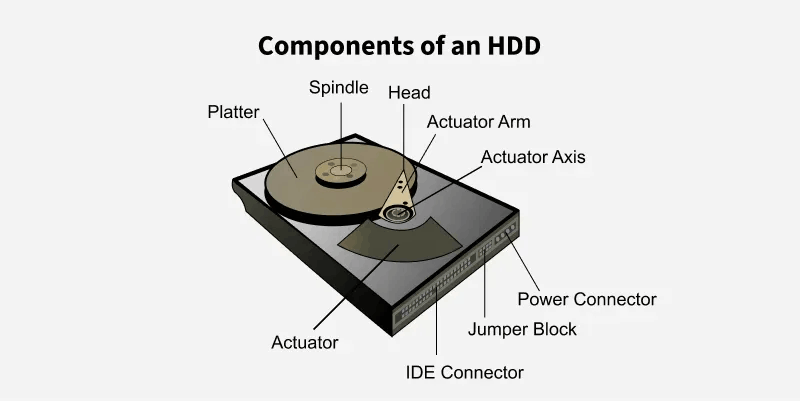
\includegraphics[width=1\linewidth]{HDD Components.png}
    \caption{Internal Components of HDD \cite{gfg_hdd_memory}}
    \label{fig:inside HDD}
\end{figure}

\newpage

\subsection{Operational Mechanism of Hard Disk Drives (HDD)}

The operation of an HDD relies on a synchronized process of mechanical rotation and magnetic signaling \cite{gfg_hdd_memory, wiki_hdd}:
\begin{enumerate}
    \item \textbf{Rotation:} The spindle motor spins the platters at high speeds, typically ranging from 4,200 to 15,000 RPM in modern drives \cite{gfg_hdd_memory, wiki_hdd}. This rotation creates an air cushion that allows the heads to "fly" nanometers above the magnetic surface \cite{wiki_hdd}.
    \item \textbf{Positioning:} When the computer requests data, the actuator arm moves the read/write head to the specific track containing the information \cite{gfg_hdd_memory, wiki_hdd}.
    \item \textbf{Magnetic Recording:} Data is stored by magnetizing the thin film on the platters. Sequential changes in the direction of magnetization represent binary data bits, often encoded using schemes like run-length limited (RLL) encoding \cite{wiki_hdd}.
    \item \textbf{Processing:} The disk controller manages the movement of the actuator, processes the raw magnetic signals into digital data using digital signal processors (DSP), and transfers it to the computer's interface \cite{gfg_hdd_memory, wiki_hdd}.
\end{enumerate}

\subsection{HDD Form Factors}

\begin{enumerate}[label=\roman*.]
    \item \textbf{3.5-inch:} The most common form factor for desktop computers and enterprise storage systems \cite{wiki_hdd, gfg_hdd_memory}. These drives typically contain one to five internal platters and are optimized for high capacity, with modern units reaching up to 36TB \cite{wiki_hdd}.
    \item \textbf{2.5-inch:} Primarily utilized in laptops, portable external drives, and some high-density servers \cite{wiki_hdd, gfg_hdd_memory}. These drives are smaller and more energy-efficient but generally offer lower total capacity than 3.5-inch models because they typically utilize fewer platters \cite{wiki_hdd}.
    \item \textbf{Enterprise Form Factors:} While physically matching 3.5-inch or 2.5-inch dimensions, enterprise-grade drives are built with specialized specifications for 24/7 operation, higher reliability, and optimized performance in server environments \cite{gfg_hdd_memory, wiki_hdd}.
    \item \textbf{Obsolete Factors:} Smaller form factors, such as 1.8-inch, 1.3-inch, 1-inch, and 0.85-inch, have been discontinued or rendered obsolete due to the superior performance and falling costs of flash memory (SSDs) in mobile devices \cite{wiki_hdd}.
\end{enumerate}


\newpage
\subsection{Limitations of HDD Technology}

\subsubsection{Mechanical Latency and Speed}
The performance of an HDD is capped by the physical movement of its components. The "Average Access Time" is restricted by:
\begin{enumerate}[label=\roman*.]
    \item \textbf{Seek Time:} The time required for the actuator arm to move the read/write head to the correct track \cite{gfg_hdd_memory, wiki_hdd}.
    \item \textbf{Rotational Latency:} The time spent waiting for the specific data sector to rotate under the head \cite{gfg_hdd_memory, wiki_hdd}.
    \item \textbf{Physical Limits:} Rotational speeds are limited by heat and vibration; while high-performance servers use 15,000 RPM drives, most consumer drives remain at 5,400 or 7,200 RPM to manage these factors \cite{wiki_hdd}.
\end{enumerate}

\subsubsection{Durability and Reliability}
Because HDDs rely on rapidly spinning platters and heads flying only nanometers above the surface, they are highly susceptible to physical failure:
\begin{enumerate}[label=\roman*.]
    \item \textbf{Fragility:} Moving parts make HDDs prone to "head crashes" if the device is dropped or subjected to physical shock, which can lead to permanent data loss \cite{gfg_hdd_memory, wiki_hdd}.
    \item \textbf{Environmental Sensitivity:} Operation can be impacted by air density; for instance, standard HDDs may fail at high altitudes (above 3,000m) because the air is too thin to provide the necessary "lift" for the heads, though sealed helium-filled drives mitigate this \cite{wiki_hdd}.
    \item \textbf{Mechanical Wear:} Over time, the spindle motors and actuator arms can wear out, leading to eventual hardware failure \cite{gfg_hdd_memory}.
\end{enumerate}

\subsubsection{Operational Overhead}
\begin{enumerate}[label=\roman*.]
    \item \textbf{Power Consumption:} The energy required to spin physical platters makes HDDs significantly less power-efficient than SSDs \cite{gfg_hdd_memory, wiki_hdd}.
    \item \textbf{Noise and Heat:} The friction and mechanical movement generate audible noise and substantial heat, requiring robust system cooling \cite{gfg_hdd_memory, wiki_hdd}.
    \item \textbf{Fragmentation:} HDDs suffer significantly from file fragmentation, where scattered data forces the read/write head to move excessively, further slowing down access times \cite{gfg_disk_mgmt, wiki_hdd}.
\end{enumerate}

\newpage
\subsection{Operating System Interaction and Management}
The Operating System (OS) interacts with the HDD through several critical management functions to ensure efficient data organization and reliable access.

\subsubsection{Formatting and File System Creation}
The OS prepares the physical disk for use through two levels of formatting:
\begin{enumerate}
    \item \textbf{Low-level (Physical) Formatting:} Usually performed at the factory, this process divides the disk into physical sectors with headers and error correction codes (ECC) \cite{gfg_disk_mgmt, wiki_hdd}.
    \item \textbf{Logical (High-level) Formatting:} The OS creates a file system (such as NTFS or ext4) and a directory structure. This defines how space is allocated and how files are retrieved \cite{gfg_disk_mgmt, wiki_hdd}.
\end{enumerate}

\subsubsection{Partitioning}
Through partitioning, the OS divides a single physical disk into multiple logical sections. Each partition acts as a separate storage device, allowing the OS to isolate the system kernel from user data or manage multiple file systems on one drive \cite{gfg_disk_mgmt}.

\subsubsection{Disk Scheduling}
Because HDDs rely on mechanical movement, the OS must manage the "Average Access Time," which is the sum of seek time (moving the head to the track) and rotational latency (waiting for the sector to rotate under the head) \cite{gfg_hdd_memory, wiki_hdd}. The OS uses disk scheduling algorithms, such as SSTF (Shortest Seek Time First) or SCAN, to determine the most efficient order for processing I/O requests, thereby minimizing mechanical wear and reducing delays \cite{gfg_disk_mgmt}.

\subsubsection{Booting and System Initialization}
When the computer is powered on, the OS bootstrap program is loaded into memory. While a small loader exists in ROM, the full bootstrap code required to initialize the system is stored in a specific "boot block" on the HDD \cite{gfg_disk_mgmt}.

\subsubsection{Error Handling and Optimization}
The OS and the disk controller work together to manage "bad sectors"---physical areas of the platter that have failed. Through a process called sector sparing, the OS remaps data from faulty sectors to spare ones in a reserve pool \cite{gfg_disk_mgmt, wiki_hdd}. Furthermore, the OS provides de-fragmentation tools to rearrange scattered file fragments into contiguous blocks, which significantly improves read/write performance by reducing unnecessary head movement \cite{gfg_disk_mgmt, wiki_hdd}.

\newpage
\begin{figure}[H]
    \centering
    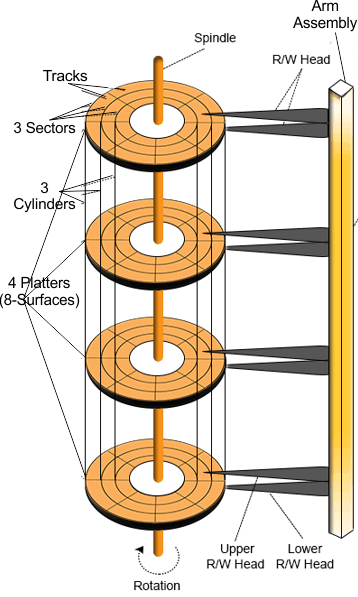
\includegraphics[width=0.7\linewidth]{OS Interaction with HDD.png}
    \caption{OS Interaction with HDD}
    \label{fig:OS and HDD}
\end{figure}

\newpage
\printbibliography
\end{document}
